\documentclass[conference]{IEEEtran}
\IEEEoverridecommandlockouts
% The preceding line is only needed to identify funding in the first footnote. If that is unneeded, please comment it out.
\usepackage{cite}
\usepackage{multirow}
\usepackage{amsmath,amssymb,amsfonts}
\usepackage{algorithmic}
\usepackage{algorithm}
\renewcommand{\algorithmicrequire}{ \textbf{Input:}} %Use Input in the format of Algorithm
\renewcommand{\algorithmicensure}{ \textbf{Output:}} %UseOutput in the format of Algorithm
\usepackage{graphicx}
\usepackage{graphicx}
\usepackage{textcomp}
\usepackage{xcolor}
\usepackage{enumerate}
\usepackage{mathrsfs}
\def\BibTeX{{\rm B\kern-.05em{\sc i\kern-.025em b}\kern-.08em
    T\kern-.1667em\lower.7ex\hbox{E}\kern-.125emX}}
\begin{document}

\title{Mobility-aware Proactive Caching Strategy in Heterogeneous Ultra-Dense Networks}

\author{\IEEEauthorblockN{Ning Gao, Xiaodong Xu, Yanzhao Hou, Lei Gao}
\IEEEauthorblockA{National Engineering Lab for Mobile Network Technologies \\
Beijing University of Posts and Telecommunications, Beijing, 100876, China\\
Email: gaoning@bupt.edu.cn}
}

\maketitle

\begin{abstract}
Caching on the wireless edge is a promising way to tackle the backhaul constraint of network densification and reduce the delay of content transmission. Although some effective caching strategies have been introduced to cellular networks, most of them ignore users' mobility, which is unreasonable. In reality, users are mobile and the associations with small-cell base stations (SBSs) can change during the file downloading, which can be more frequent in heterogeneous ultra-dense networks (H-UDNs). Files missing in a new SBS will greatly increase the delay of file transmission. In this paper, we propose a mobility-aware proactive caching strategy in H-UDNs, which can proactively schedule contents between different cache layers to improve users’ quality of service (QoS) as well as cache hit ratio. The cache placement problem is formulated with the aim of effective capacity maximization and solved by a genetic algorithm (GA)-based approach. Simulation results show that the proposed caching strategy outperforms the most popular caching (MPC) strategy.
\end{abstract}

\begin{IEEEkeywords}
 Mobility, caching strategy, heterogeneous ultra-dense networks (H-UDNs), effective capacity, genetic algorithm
\end{IEEEkeywords}

\section{Introduction}
With the rapid development of mobile Internet, a large number of new applications are widely applied, such as AR/VR and online games. These applications require the mobile network to provide higher data transmission rate and lower network delay. Moreover, it is predicted that the mobile data traffic will reach 30.6 exabytes/month globally by year 2020\cite{cisco}. To handle these challenges, heterogeneous ultra-dense networks (H-UDNs) with dense small-cell base stations (SBSs) and macro base station (MBS) have been introduced to enhance the network capacity. However, the costly and heavily-loaded backhaul link between H-UDNs and the core network is becoming the bottleneck\cite{6963798}.

Caching in the H-UDNs has been widely recognized as an effective and economical solution to tackle the aforementioned challenges. By storing popular files in the densely deployed SBSs in advance \cite{8269405}, more requests can be satisfied at SBSs instead of retrieving duplicated files over the backhaul links. Besides, downloading directly from SBSs can reduces delay substantially due to the short transmission distance \cite{6736753}. However, the storage capacity on SBSs is usually limited, and thus caching strategies should be carefully designed to make the best use of the SBSs cache.

There have been some recent works focusing on designing caching strategies in the scenario of H-UDNs. The auther of \cite{6600983} present a wireless distributed caching strategy with a low-bandwidth backhaul link but high storage capacity where users can access multiple SBSs. Finding the optimal cache placement to maximize cache hit ratio is proved to be NP-complete. The authors of \cite{6952688} study the optimization issue for cache content placement in cache-enabled H-UDNs with heterogeneous files and cache sizes and adopt multicast transmission to minimize the average backhaul rate. In the work of \cite{8116421}, the authors propose a cooperative caching strategy where SBSs can get the desired content from neighboring SBSs so as to enhance the content delivery efficiency.

Although these recent works have provided insight into caching strategy cellular networks, users are assumed to be static and the association between users and SBSs remains unchanged. Obviously, such an assumption is unreasonable in mobile celluar networks. In fact, users are moving and the associations to SBSs can change during the file downloading, which can be more frequently in H-UDNs \cite{7268835}. The cache placement policy which ignores user mobility cannot capture the spatial distribution changes of users' requests in time and causes a lower degree of matching between files and request. Therefore, the impact of user mobility cannot be neglect when designing file caching strategies \cite{7537180}. Reference \cite{8013789} uses a discrete random jump model to describe the mobility pattern and derive the expression of throughput. Due to the complexity of the problem, two heuristic algorithms are provided to obtain the optimal solution. The author of \cite{6620380} assumes that the user movement obeys a discrete Markov model and the amount of data downloaded by users depends on their location and the cache placement in each time slot. The user mobility is also modeled as Markov chain and a distributed caching strategy is proposed in a two-tier heterogeneous network with the aim of minimizing the content fetched from the MBS \cite{7484297}.

Although these works have taken user mobility into account, they have not fully utilized the hierarchical architecture of heterogeneous networks to address the problems caused by user mobility. In a cache-enabled H-UDN, both MBS and SBS can storage files but the file transmission delay is different. SBSs are close to the user with a small delay while the MBS is relatively far form users with a slightly larger delay. And the requests that SBSs miss are redirected to the MBS \cite{7484297}. Assuming that the user only accesses SBSs, the high-speed movement will cause the user to frequently switch between multiple SBSs. Due to the randomness of user movement, it is very difficult to push the required files to SBSs accurately in advance to reduce the delay, and the cache hit ratio is hard to guarantee. On the contrary, if these contents are more likely to be cached in the MBS, the cache hit rate of high-speed users can be effectively improved at the cost of a slightly larger delay. In addition, the SBSs can store more other content to satisfy more low-speed users' content requests.

In this paper, we are motivated to propose a mobility-aware proactive caching strategy to improve users’ quality of service (QoS) and cache hit ratio. Files can be scheduled between different cache layer depending on user mobility. The contributions of this paper include:

\begin{enumerate} [1)]
 \item We propose a mobility-aware proactive caching strategy in H-UDNs to provide the mobile users with better QoS.
 \item  The cache placement problem is formulated as a 0-1 integer nonlinear programming problem with the aim of effective capacity maximization, which can reflect the impact of delay in user data rate.
 \item We solve the problem by a genetic algorithm (GA)-based approach. Simulation results show that the proposed strategy can achieve better performance compared with the most popular caching (MPC) strategy.
\end{enumerate}

The remainder of this paper is organized as follows. Section II describes the system model, including network model, file popularity model, mobility model and effective capacity based QoS parameter. In Section III, we introduce the proposed mobility-aware proactive caching strategy and solve the cache placement problem with the GA-based approach. In Section IV, numerical results are illustrated with performance comparisons between MPC. Finally, conclusions are summarized in Section V.

\section{System Model}
\subsection{Network Model}
In this paper, we consider a cache-enabled heterogeneous network comprising a single MBS and $K$ densely deployed SBS denoted as $\mathcal{K} \triangleq\{0\mathrm{,\,}1\mathrm{,\,}2\mathrm{,\,}...\mathrm{,\,}K\}$, where $\mathcal{K}_0$ represents the MBS. In this scenario, the MBS and SBSs are connected by a fronthaul link with the limited capacity of $r_{FH}$ and the MBS is connected to the core network by a backhaul link with the lcapacity of $ r_{BH}$. The set of active users is denoted as $\mathcal{U} \triangleq\{1\mathrm{,\,}2\mathrm{,\,}3\mathrm{,\,}...\mathrm{,\,}U\}$ and each user $u$ only connects to and receives data from the nearest SBS (in terms of signal strength), which we later refer to as the  home-SBS of user \emph{u}. And the number of users associate with SBS $i$ is denoted as $U_i$.

%fig 1
\begin{figure}[htbp]
 \centerline{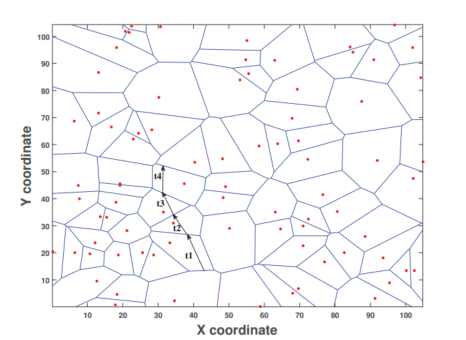
\includegraphics[scale=0.5]{fig1.png}}
 \caption{System model and file delivery.}
 \label{fig 1}
\end{figure}

\subsection{Cache File Model}
We assume that the MBS has access to a library of $\mathrm{F}$ files denoted as $\mathcal{F} \triangleq\{1\mathrm{,\,}2\mathrm{,\,}3...\mathrm{,\,}F\}$, and each file has the same size denoted by $B$ [MB]. Note that the assumption of equal size files is justifiable in practice since files can be divided into blocks of the same size.

We assume that SBS $i$ are equipped whih a cache to storage files with storage capacity of $C_i$ [MB], and the MBS is equipped with a large cache with storage capacity of $C_0$ [MB]. Each user requesting for files in $\mathcal{F}$ is initially served by the home-SBS. If the requested file is not present in the cache, other SBSs nearby or the MBS will send the file to the user as shown in Fig.1. To describe the cache placement, we define the binary placement matrix as
$$\mathcal{X}=
\begin{Bmatrix}
x_{0,1}    &x_{0,2}  & \cdots & x_{0,F} \\
x_{1,1}    &x_{1,2}  & \cdots & x_{1,F} \\
\vdots    &\vdots  & \ddots &\vdots \\
x_{K,1}    &x_{K,2}  & \cdots & x_{K,F}
\end{Bmatrix}
$$
where $x_{i,j}=1$ denotes the file $f_j$ is cached in the base station (BS) $i$ and $x_{i,j}=0$ denotes the file $f_j$ is not cached in BS $i$. Note that the indexing $i$ of $x_{i,j}\mathrm{,\,} i=0,1,...,K$, includes all the MBS and SBSs. The cache storage capacity constraints can be expressed as

\begin{equation}
\sum_{j=0}^F B\cdot x_{i,j}<C_i,\forall{i}\in\mathcal{K}
\end{equation}

Moreover, we define the popularity of files in BS $i$ as $\mathcal{P} \triangleq\{p_{i,1}\mathrm{,\,}p_{i,2}\mathrm{,\,}p_{i,3}...\mathrm{,\,}p_{i,F}\}$, in which $p_{i,j}$ is the probability of the file $f_j$ being requested from a user in BSs $i$, and $ \sum_{j=1}^N p_{i,j}=1,\,\forall{i}\in\mathcal{K}$. It should be noted that the content popularity here is inferred with historical data by least commonly used algorithm (LFU) and may not reflect the file request probability in the next time period due to user mobility.

\subsection{Mobility Model}
User mobility is modeled by discrete random jumps, with the corresponding intensity characterized by average sojourn time. In terms of the distribution of sojourn time, it is reasonable to model it by an exponential function\cite{8013789}. Therefore, the probability density function (PDF) of sojourn time in SBS $i$ can be written as follows
\begin{equation}
p(\tau,\mu)=\frac{1}{\mu}e^{-\tau/\mu}
\end{equation}
where $\mu$ is the average sojourn time. A small $\mu$ indicates intense mobility and vice versa.

In addition, in order to predict the trajectory of moving users, we adopt the stationary Markov chain model and use $T_{l,i}\ge 0$ to denote the transition probability from SBS $l$ to SBS $i$, which can be predicted by machine learning techniques roughly in reality.

\subsection{Effective Capacity based QoS parameter}
Although introducing caching technology into H-UDN shortens the access distance between users and contents significantly, it is not easy to find a proper measure to evaluate this advantage. Conventional channel models are formed from the perspective of physical layer, so it is difficult to evaluate the QoS supporting ability of the channel, such as bounds on delay and packet loss ratio. In \cite{1210731}, the authors construct the channel model from the link layer and analyze the behavior of the connection under complex QoS requirements with the queuing theory. The maximum arrival rate the wireless channel can supported is defined as a log-moment generation function as follow
\begin{equation}
\alpha(\theta)=-\lim_{t \to \infty}\frac{1}{\theta t}\log E\{e^{-\theta S(t)}\}
\end{equation}
where $S(t)=\int_{0}^{t} r(t)\, dt$ represents the data throughput accumulated on the time domain. Considering the scenario that channel coefficients keep constant over the frame duration T and vary independently for each frame, the formula of effective capacity can be rewritten as follow
\begin{equation}
\alpha(\theta)=-\lim_{t \to \infty}\frac{1}{\theta t}\log E\{e^{-\theta TR[i]}\}
\end{equation}
where $R[i]$ indicates the instantaneous channel capacity during the $i$th frame.

Due to the time-varying and randomness of wireless channels, deterministic delay guarantees for specific links are unreasonable and impractical. So, the effective capacity denotes
$\theta$as the statistical QoS guarantee parameter and the delay violation possibility can be written as
\begin{equation}
Pr\{D(\infty)>D_{max}\}\approx e^{-\theta D_{max}}
\end{equation}
where $D_{max}$ indicates the delay bound and a larger $\theta$ represents a better link quality or a tighter QoS constraints. Note that when $\theta$ approaches to zero, the effective capacity converges to the ergodic capability.

According to the queuing theory, the queue delay $D(\infty)$ of the packet satisfies the following relation \cite{1363841}.
\begin{equation}
\theta=-\lim_{D_{max}\to \infty}\frac{\log(Pr\{D(\infty)>D_{max}\})}{D_{max}-\sum_h d_h}
\end{equation}
where $d_h$ is the transmission delay caused by the h-hop in data packet ransmission.

In the scenario of this paper, the transmission delay can be different accroding to where user can get the requested file. When the user requested file is not avalilable in the home-SBS, it has to retrieve it from other places. The transmission delay of transfering a file from MBS to home-SBS via fronthaul link is $d_0={B}/{r_{FH}}$. And, sharing files between neighbor-SBS $l$ and home-SBS i will cause different transmission delay depending on the hops number $h_{l,i}$, which can be denoted by $d_{l,i}=h_{l,i}{B}/{r_{FH}}$. Furthermore, retrieving the file from the core network through the backhaul link generally results in a large transmission delay $d_c=h_c{B}/{r_{BH}}$ with additional $h_c$ hops. In practice, $d_c$ is usually of many-fold higher than $d_0$ and $d_{l,i}$, which makes it cost-effective to retrieve files from the in-netwok caches rather than downloading them from the core network \cite{6736753}.

The place where user can get the requested file affects the effective capacity of the wireless link, as the value of the QoS guarantee factor changes according to $x_{i,j}$. Thus given a cache placement matrix $\mathcal{X}$, we can get the average transmission delay of user \emph{u} in cell \emph{i} for file \emph{j} as
\begin{equation}
d_{u,i,j}=(1-x_{i,j})(x_{0,j}d_0+\frac{1-x_{0,j}}{K-2}\sum_{l\in S\setminus{\{0,i\}}}x_{l,j}d_{l,i})+c_jd_c
\end{equation}
where $c_j= \prod_{i\in \mathcal{S}}(1-x_{i,j})$, which means the file $j$ is not storaged in the H-UDN.

Substituting $d_{u,i,j}$ to equation (6), the QoS guarantee parameter can be expressed as
\begin{equation}
\theta_{u,i,j}=-\lim_{D_{max}\to \infty}\frac{\log(Pr\{D(\infty)>D_{max}\})}{D_{max}- d_{u,i,j}}
\end{equation}

\section{GA-based Mobility-aware Proactive Caching Strategy}
Here, we first explore the impact of user mobility on file popularity of different BSs. Then, we formulate the cache placement optimization problem aimed at effective capacity maximization. Finally, a GA-based approache is introduced to solve this problem.
\subsection{Mobility-aware content request probability}
When a user arrives at SBS $l$ with an incomplete downloading of content $j$, part of the file $B_{l,j}$ has been downloaded already. Hence the user only needs to download the rest of the content $j$. For simplicity, we assume the maximum bandwidth of $G$ [MB/s] of each SBS is shared equally among the associated users of that SBS\cite{8108779}. Thus, the bandwidth allocated to each user connecting to SBS $l$ is given by $r_l=G/U_l$.

Since each content file has $B$ MB, the time needed to completely download one content at SBS $l$ is $t_l=B/r_l$.
However, the sojourn time that user stays in SBS $l$ is subject to exponential distribution, so the probability of the user completing the download when leaving the SBS $l$ can be inferred using the Cumulative Distribution Function $F(\tau,\mu)$ as,
\begin{equation}
  \begin{aligned}
 q_{l,j}=& Pr(\tau<t_l-\frac{B_{l,j}}{r_l})\\
  &=F(t_l-\frac{B_{l,j}}{r_l})\\
  &=1-exp(-(t_l-\frac{B_{l,j}}{r_l}/\mu)
  \end{aligned}
\end{equation}

Then, the file requested probability ${\tilde{p}_{i,j}}$ with user mobility of content $j$ at BS $i$ can be predicted as
\begin{equation}
{\tilde{p}_{i,j}}=
\begin{cases}
p_{i,j}+\lambda\sum_{l\neq i}p_{l,j}q_{l,j},  & i=0\\
p_{i,j}+(1-\lambda)\sum_{l\neq i}p_{l,j}q_{l,j}T_{l,j}, & i\in S\setminus\{0\}
\end{cases}
\end{equation}
where $p_{i,j}$ is the prior popularity of file $j$ at BS $i$ and $T_{l,i}$ is the transition probability from SBS $l$ to $i$. The  $\lambda\in(0,1)$ is a weighting factor to balance the tradeoff between the SBS cache and MBS cache. A larger $\lambda$ will make files tend to be cached in the MBS cache, voiding retrieving files from the core network caused by frequent handovers among SBSs. Conversely, a smaller $\lambda$ factor will make files tend to be cached in SBSs, minimizing the transmission delay.

\subsection{Problem Formulation}
Based on the system model and effective capacity theory previously mentioned, the effective capacity achieved by user $u$ in SBS $i$ can be expressed by the following formulation
\begin{equation}
\alpha_{u,i}(\theta)=\sum_j{\tilde{p}_{i,j}}(-\frac{1}{\theta_{u,i,j}T}\log E\{e^{-\theta_{u,i,j}Tr_i}\})
\end{equation}
Then, the cache placement problem can be formulated as follows with the purpose of maximizing the total effective capacity of the whole system.
\begin{equation}
 \begin{aligned}
   & {max}\ \sum_u\sum_i\alpha_{u,i}(\theta)\\
   & s.t. \quad\sum B\cdot x_{i,j}<C_i\\
   & \qquad \ x_{i,j}\in\{0,1\}
 \end{aligned}
\end{equation}

Obviously, the optimal problem is a 0-1 integer nonlinear programming problem which is highly complicated to obtain a close-form solution. Therefore, a GA-based approach is introduced to solve this problem in the next section.

\subsection{The GA-based approach}
The Genetic algorithm is an adaptive heuristic search algorithm based on the evolutionary ideas of natural selection, and it is inherently suitable for solving optimization problems with binary variables \cite{Srinivas2002Genetic}.

Firstly, the initial population including $N_p$ candidate caching placement matrices is grenerated, and each matrix is called an individual. Then the objective value of each individual is calculated through equation (11). $N_e$ individuals with top objective values are chosen as elites and pass into the next generation directly. The rest of the next generation population are generated through crossover and mutation operations. The crossover function selects two individuals parent individuals to generate two crossover children, and the mutation function just operates on a single individual and generates a mutation child. The numbers of individuals generated through crossover and mutation operations are denoted as $N_c$ and $N_m$ , respectively, where $N_e+N_c+N_m=N_p$ and the crossover fraction is $f_c=N_c/ (N_c+N_m)$. Roulette wheel selection is adopted, and individuals with higher objective values in current generations will have a higher probability to generate offsprings. Repeat the evaluation-selection-generation procedures until Ng generation is created. Finally, the best individual in the current population is chosen as the output of the algorithm. The initial population, crossover function and mutation function of the proposed GA approach are described as follows.

1)	Initial Population: The initial population is created as a set of $\mathcal{X}^{(K+1)F}$. For each row in each individual, $M_i$ of the $F$ elements are set to be 1 randomly, and all the left elements are set to 0, where

\begin{equation}
\sum_{i=0}^K B\cdot M_i <C_i, \forall{i}\in\mathcal{K}
\end{equation}
for the storage capacity constraint in each BS.

2)	Crossover Function: The crossover function use a two-point crossover function to generate one children, which is described in Algorithm 1. The steps 5-10 are heuristic processes to meet constraint (13).

3)	Mutation Function:  For each row of the individual, one of $F$ elements is randomly selected and the value is set to be the opposite. The mutation operation reduces the probability that the algorithm converges to local minimums.

The complexity of the proposed GA-based approach is $N_p\cdot N_g$, where $ N_p$ and $N_g$ are the population size and terminal generations number, respectively.

\begin{algorithm}[htb]
 \caption{Crossover function}
 \label{alg:admission}
 \begin{algorithmic}[1] %这个1 表示每一行都显示数字
 \STATE Get parent $\mathcal{X}_1=\{x_{i,j}^{(1)}\}$ and $\mathcal{X}_2=\{x_{i,j}^{(2)}\}$,  initialize their child  $\mathcal{X}_c=\{x_{i,j}^{(c)}\}$
\FOR{$i=0,1,\cdots,K$}
\STATE{Generate random integers $j_1, j_2 \in[1, F]$, $j_1 < j_2$}
\STATE{Replace $x_{i,j}^{(1)}, j=\{j_1,j_1+1,\cdots,j_2\}$ of $\mathcal{X}_1$ with $x_{i,j}^{(2)}, j=\{j_1,j_1+1,\cdots,j_2\}$ of $\mathcal X_2$, and then set $x_{i,j}^{(c)}=x_{i,j}^{(1)}, \forall j\in\{1,2,\cdots,F\}$.}
\WHILE{$\sum_{j=1}^{F} x_{i,j}^{(c)}>M_i$}
\STATE{Set nonzero $x_{i,j}^{(c)}$ to 0 in descending order of $j$}.
\ENDWHILE
\WHILE{$\sum_{j=1}^{F} x_{i,j}^{(c)}<M_i$}
\STATE{Set zero $x_{i,j}^{(c)}$ to 1 in ascending order of $j$}.
\ENDWHILE
\ENDFOR
\end{algorithmic}
\end{algorithm}

\section{Performance Evaluation}
In this section, we use computer simulation methods to evaluate the performance of the mobility-aware proactive caching strategy for H-UDNs. We simulated a H-UDN depicted in Fig1, where an MBS is located in the center and multiple SBSs are uniformly deployed in the network. Several moving users are randomly distributed in the network and we consider a wrap-around network layout such that when a user moves out of the network on one side, it comes back in on the opposite side w.r.t. the origin. In addition, we assume that the files users request can be modeled as the Zipf distribution\cite{6736753}. The request probability of file $f_j$ is
$$p_j=\frac{1/j^\gamma}{\sum_{j=1}^F 1/j^\gamma}, \forall j\in F$$
where $\gamma$ is the skewness reflecting the concentration of the popularity distribution among users. All other simulation parameters are listed in Tabel 1.

\begin{table}[htbp]
 \caption{Simulation Parameters}
 \setlength{\tabcolsep}{7mm}
 \begin{center}
  \begin{tabular}{|l|c|}
   \hline
   \multicolumn{2}{|c|}{System Parameter}                \\\hline
   Number of MBS                  & 1                 \\ \hline
   Number of SBSs $K$             & 100                \\\hline
   Fronthaul rate $r_{FH}$        & 600Mbps               \\ \hline
   Backhaul rate $r_{BH}$         & 1000Mbps               \\\hline
   Bandwidth of SBS $G$           &  100Mbps              \\\hline
   Number of Files $F$            & 200               \\\hline
   Size of Files $B$              & 50MB            \\\hline
   \multicolumn{2}{|c|}{GA Parameter}                \\\hline
   Population size $N_p$          & 50              \\\hline
   Terminal generation number $N_g$ & 100               \\\hline
   Number of elites $N_e$         & 10              \\\hline
   Crossover fractio $f_c$        & 0.8            \\\hline
  \end{tabular}
  \label{tab1}
 \end{center}
\end{table}

We compare the performance of our optimal caching scheme with MPC schemes which uses global static content popularity and each BS stores the most popular files until its cache is full\cite{6600983}.
\subsection{Capacity Based System Tthroughput Performance}
  Fig.\ref{fig 3} shows the effective capacity based system throughput when the num of users varies in the network, where we set $\gamma=0.7$ and $\mu=4$. Obviously, we see that as the number of users increases, the system throughout improves and the mobility-aware proactive caching strategy always outperforms the MPC strategy. This is because that files cached in the SBSs and MBS changes according to users’ location and preference. Hence, it can match the user request better and reduce the transmission delay.
\begin{figure}[htbp]
 \centerline{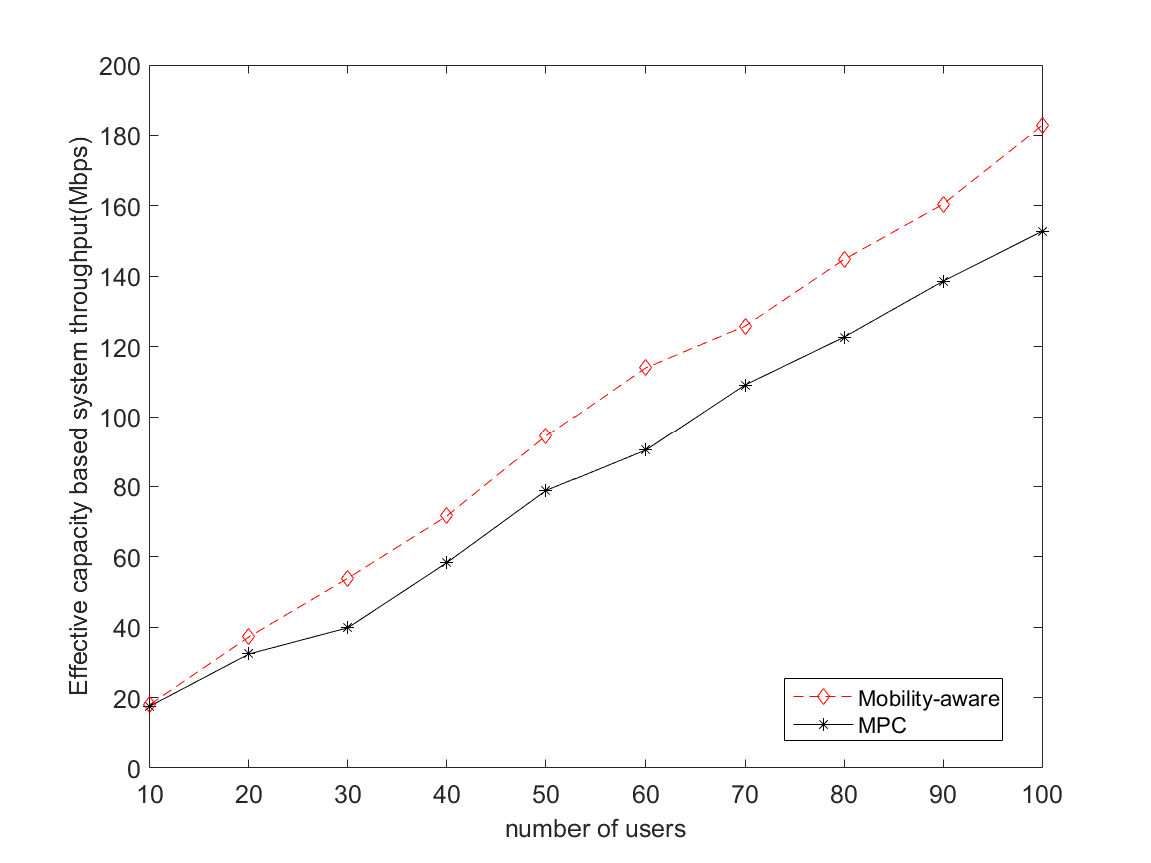
\includegraphics[scale=0.35]{fig3.png}}
 \caption{System throughput gain with the proposed caching strategy}
 \label{fig 3}
\end{figure}
Fig.\ref{fig 4} investigate the relationship between cache size and system throughput. As shown in Fig.\ref{fig 4}, with the increasing of total cache size, the effective capacity based system throughput gains at the same time. It demonstrates the fact that expense of storage can alleviate the shortage of backhaul bandwidth and improve the data rate that a user achieves. The more contents BSs store, the more chances users can get the contents in H-UDNs so that they can be served immediately.
\begin{figure}[htbp]
 \centerline{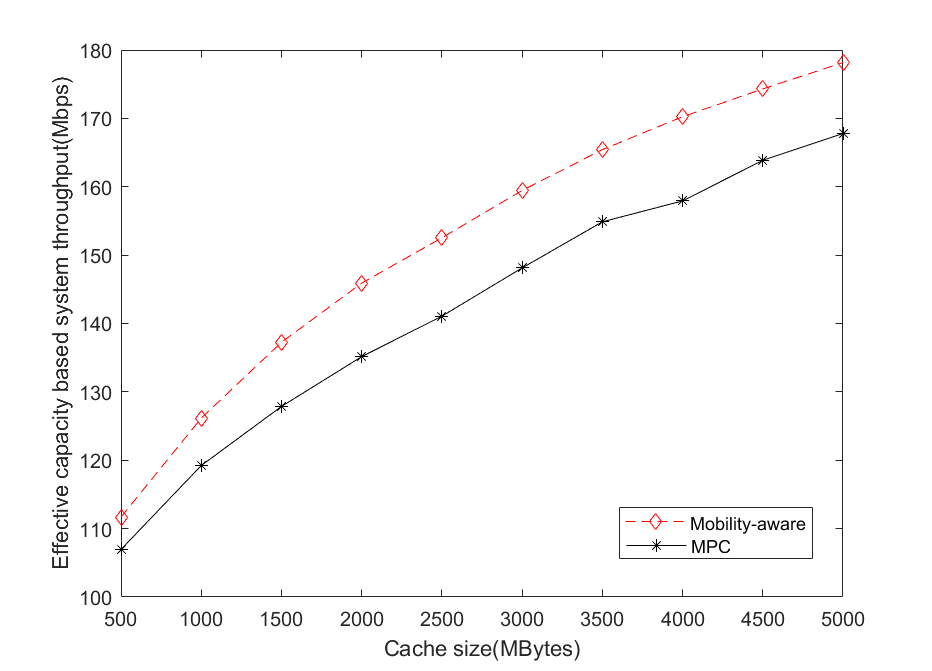
\includegraphics[scale=0.3]{fig4.png}}
 \caption{System throughput versus cache capacity}
 \label{fig 4}
\end{figure}
\subsection{Cache Hit Ratio Performance}
Fig.\ref{fig 5} displays the impact of file populatity distribution parameter $\gamma$ on the cache hit ratio. In this simulation, user number is set to 70. As the figure shows, when $\gamma$ is small, both two caching strategy have low cache hit ratio. Because in this case, all files are almost equally likely to be requested but the storage capacity of BSs is limited. In this case, mobility-aware caching strategy still achieves superior performance than MPC. When $\gamma$ becomes larger, the requests are more concentrated among some popular files. Therefore, these popular files are more likely to be stored in most SBSs to satisfy more user requests. Hence the caching hit ratio of mobility-aware and MPC both improve notably.
\begin{figure}[htbp]
 \centerline{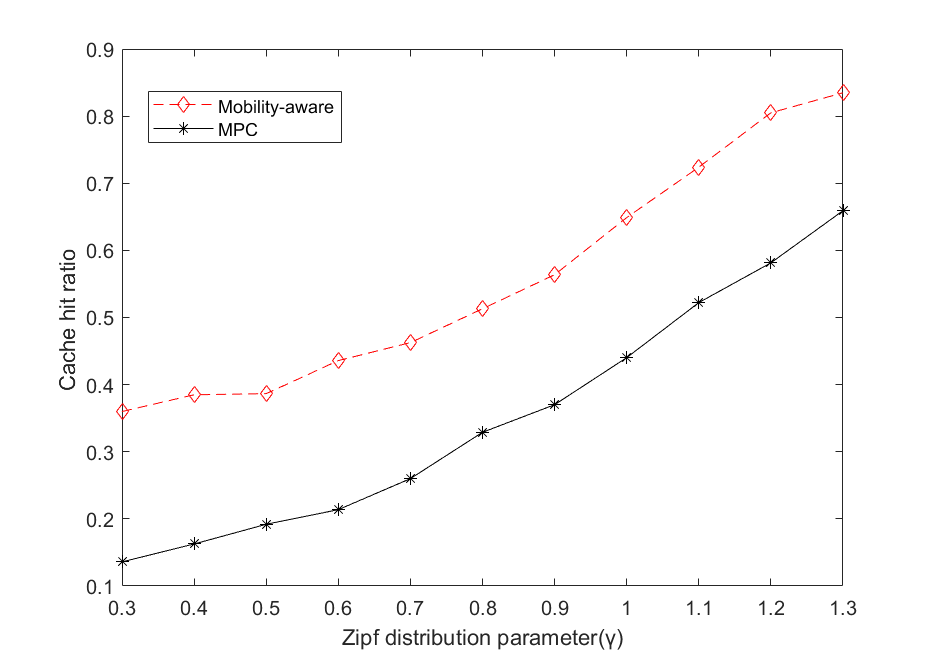
\includegraphics[scale=0.3]{fig5.png}}
 \caption{Cache hit ratio as a function of Zipf distribution parameter $\gamma$ }
 \label{fig 5}
\end{figure}
\section{Conclusion}

In this paper, we propose a new mobility-aware proactive caching strategy in H-UDNs and use the effective capacity to evaluate the effect of transmission delay on user data rate. We use random jump model and stationary Markov chain model jointly to describe the mobile pattern of users and use it to predict the file popularity at MBS and SBSs. Then, the optimal content placement problem is formulated as a 0-1 integer nonlinear programming problem and solved by the GA-based approach. Finally, simulation results show that the proposed mobility-aware proactive caching strategy achieves better QoS and cache hit ratio than MPC strategy.

\section*{Acknowledgment}

This paper is supported by Beijing Municipal S\&T project Z181100003218003, Nature and Science Foundation of China No. 61871045 and 111 Project of China B16006.

\bibliographystyle{IEEEtran}
\bibliography{reference}
\end{document}
